\section{What is Reinforcement Learning?}

\textbf{Reinforcement learning (RL)} is a subset of machine learning that has its origins in computer science and artificial intelligence techniques established in the 1950s.
RL is unique within machine learning as it is focused on goal-directed learning from agent-environment interaction\cite{rlai}.
Simply put, agents learn from environment interactions and gain experience.
They use this experience to optimize their behaviour to achieve problem-defined goals.
This nature-inspired approach captures a broader definition of intelligence (in a human sense) than systems that reason about the world using a finite set of logical rules (i.e., knowledge-based systems).
Like most other subfields of ML, RL is a class of problems as well as a class of solutions to those problems\cite{rlai}.

Advances in the field of deep learning (a broad family of methods based on artificial neural networks\cite{wiki:Deep_learning}) that could enhance the classical algorithms used in RL led to the expansion of the field -- marking the birth of \textbf{deep reinforcement learning (deep RL)}.
Deep RL has surged recently after a series of new algorithms and succesful applications were released. In the following paragraphs, we will summarize some of the most significant results.

\textbf{AlphaGo} (2015)\cite{ago} managed superhuman performance in the game of Go, beating 18-time world champion Lee Sedol.
In late 2017, the AlphaGo family was expanded to contain AlphaGo Zero and AlphaZero\cite{azero}.
Both systems have managed to surpass all their predecessors in game performance, as well as training efficiency \cite{wiki:AlphaGo} (a lot less training time was required to beat the record).
The key difference was that their training was done with absolutely no expert knowledge for either system (hence the ``zero'').
Instead, everything was learned by self-play \cite{azero}.

\textit{Mnih et al.}'s \textbf{DQN}\cite{atari-dqn} (2013) managed impressive performance at seven classic Atari games.
The agents learn solely by observing the screen, without being given game-specific information.
This study produced agents able to surpass human-level performance in \emph{Breakout}, \emph{Enduro} and \emph{Pong}.
Following the success of DQN, the community worked to improve the standard algorithms, such as DDQN \cite{ddqn-paper} and PER \cite{per-paper}.
In Rainbow DQN (2017)\cite{rainbow-dqn}, the authors succesfully combined multiple high-quality improvement methods over the original DQN.
The resulting algorithm set a new record on the Atari benchmark.

\textbf{OpenAI Five}\cite{openai-dota} (2018) produced a bot that managed to beat top professional Dota 2 players in international championships.

Despite most of the above list being focused on achievements in video games, RL has been applied to other problems including robot control, elevator scheduling, telecommunications\cite{wiki:Reinforcement_learning}.

\section{Fundamental Components}

First of all, we present the agent-environment feedback loop, as it is crucial to understand the dynamic. An agent acts upon the environment, which reacts according to its set of governing rules.
\begin{enumerate}
    \item The agent receives a reward for this action. This (immediate) reward signal is problem-defined and quantifies the agent’s goal. (see the Reward Hypothesis).
    \item The environment reaction sends the agent into the next state.
    \item The agent perceives and needs to decide on its next action.
\end{enumerate}

\begin{figure}[h]
    \caption{The interaction loop. (Partial reproduction from \cite{rlai}, 3.2)}
    \centering
    \vspace*{0.5cm}
    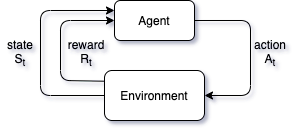
\includegraphics[width=0.5\textwidth]{agent-env-fig}
\end{figure}

\subsection{State and Policy}

We use the concept of \textbf{state}. The state most often refers to the internal state of the agent. Although, in some contexts, we can use it to mean the environment state.
A state contains relevant information from the environment at a given time-step.
A key point in RL is that a well-engineered (agent) state captures all the relevant information and removes the need of explicitly memorizing state history.
This is mathematically by described the \textbf{Markov property}\cite{silver-lectures}, a fundamental property of the mathematical framework underpinning RL -- Markov decision processes (MDPs).

A \textbf{policy} completely characterizes the agent’s behaviour.
``It is a mapping from perceived states of the environment to actions to be taken in those states'' \cite{rlai}.
Policies can be deterministic (i.e. ``if this then that'' rules) or stochastic.
A \textbf{stochastic policy}\cite{silver-lectures} is a probability distribution over actions, given a state.

\subsection{Reward}
``The reward signal is the primary basis of altering the policy.'' \cite{rlai}.
The \textbf{reward} models the problem-defined goals as a scalar that can be associated with each state transition.
The assertion that we can completely and correctly model all goals using reward functions is central to the field of RL.
This is called the \textbf{Reward Hypothesis} and is formulated below:
\begin{quotation}
    That all of what we mean by goals and purposes can be well thought of as maximization of the expected value of the cumulative sum of a received scalar signal (called reward). \textit{(from \cite{rlai}, Chapter 3.2)}
\end{quotation}

The \textbf{return} denotes the cumulative reward obtained by the agent over time.
This is what a RL system is supposed to maximize.
There are multiple mathematical models used to represent the return.
The simplest example is to simply sum the reward over a finite number of steps.
However, in practice we often use \textbf{discounting}.
Discounting is, simply, a way to control how much the agent cares about future rewards.
More on this topic can be found in either theorethical reference \cite{rlai,silver-lectures}.
% In the actual paper, elaborate here.

\subsection{Value Function}\label{rl:value-func}

A \textbf{value function} measures how good each state is, with regard to the long-term potential of that state.
``Whereas rewards define the immediate desirability of an environmental state'', a value function ``indicates the long-term desirability of a state'' \cite{rlai}.
The value of a state is given by two things:
\begin{enumerate}
    \item the immediate value of being in that state (that state’s immediate reward)
    \item the potential return going forward in time from that state.
\end{enumerate}

This models a \textbf{long-term thinking aspect} into learning, as choosing one state over another often excludes future paths of action.
Let us take a game of chess as example.
If one move leads to the opponent capturing one of the agent's pieces, no future actions can be executed with that piece.
Thus, making a move with a high initial reward (for example, the agent trades a pawn for a knight), excludes -- for example -- the option of \textbf{promoting} that particular pawn (a later, higher reward).

\subsection{Model}
A RL system may or may not have a \textbf{model}.
A \textbf{model} (of the environment) allows the agent to plan and make predictions of its environment.

Some algorithms focus explicitly on learning a model and use it for \emph{planning}.
This approach is called \textbf{model-based}.
In this case, an agent can query the model to simulate what would happen with the environment, before actually choosing an action (hence the planning aspect).

Approaches without a model are called \textbf{model-free}.
Model-free agents are ``explicitly trial-and-error learners'' \cite{rlai}.

\begin{figure}[ht]
    \caption{A way of classifying RL methods based on whether it has a value function, policy or model. (Reproduced from David Silver's lectures. \cite{silver-lectures})}
    \vspace*{0.2cm}
    \centering
    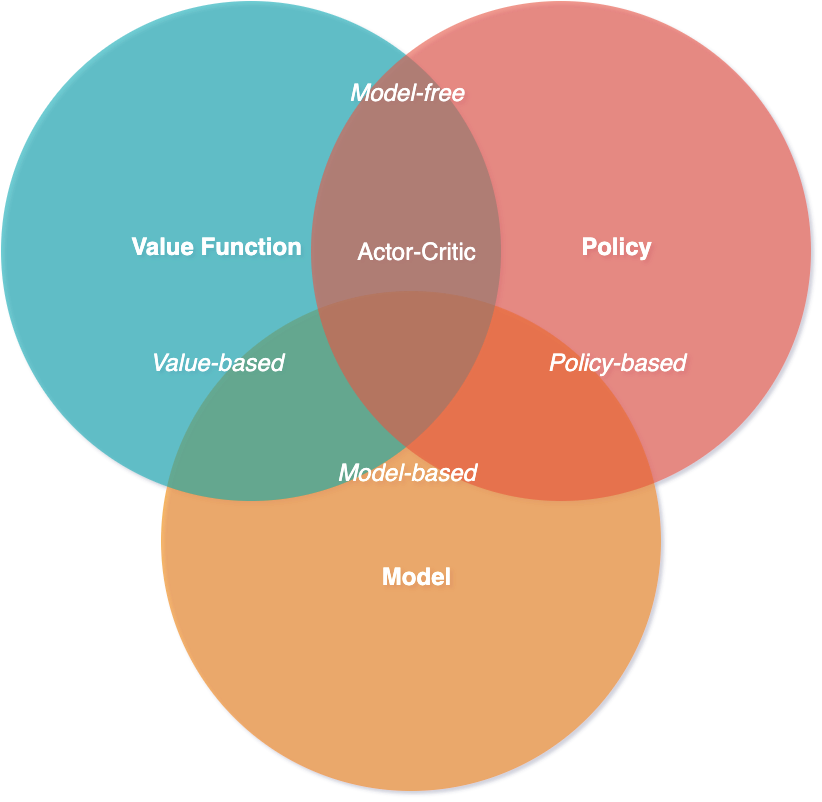
\includegraphics[width=0.65\textwidth]{silver-venn}
\end{figure}
